\documentclass[paper-main.tex]{subfiles}

\begin{document}

\begin{figure}
	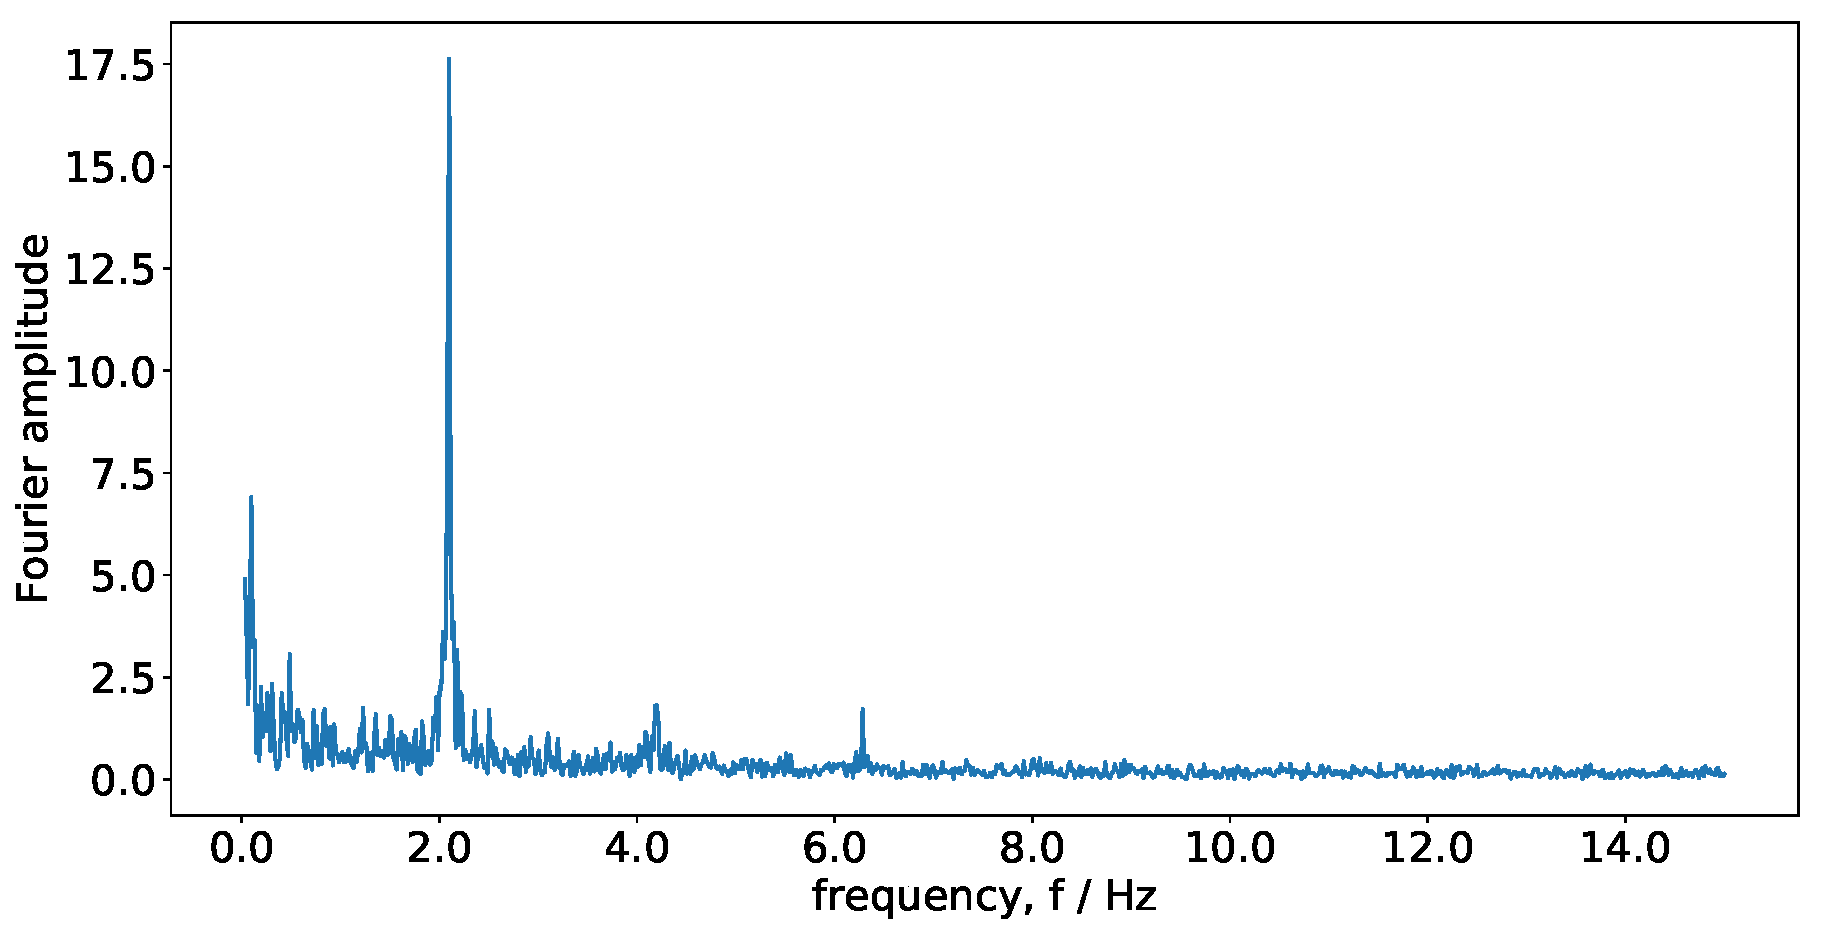
\includegraphics[width=.49\textwidth]{figures/webcam_expt_4_0209-cropped.pdf}
	\caption{\label{fig:webcam_spectrum}
Injected tone at a constant frequency: Fourier amplitude of the intensity time series recorded by the webcam. 
The frequency of the injection is $2.09\,{\rm Hz}$. 
The recovered signal peaks at $2.099\,{\rm Hz}$ with a FWHM of $0.033\,{\rm Hz}$. 
There are also two visible harmonic peaks at integer multiples of the main peak. 
Their amplitudes as a fraction of the height of the main peak are  $0.103$ and $0.098$ for the $4.19\,{\rm Hz}$ and $6.28\,{\rm Hz}$ peaks respectively. 
}
	
\end{figure}


Continuous-wave searches look for signals which are close to monochromatic. 
In this section we consider a simple sinusoidal tone; a note at a single constant frequency. 
As described in Section~\ref{sec:ifo}, the audio is played through a speaker fixed to the back of one of the mirrors.


The intensity of the interference pattern is measured at a single point on the screen using a commercial USB webcam placed to view the screen (see Fig.~\ref{fig:ifo_schematic_webcam}). 
The webcam's sample rate is $30\,{\rm Hz}$, which limits the spectral content of observable signals to below $15\,{\rm Hz}$, the Nyquist frequency.
A tone under $15\,{\rm Hz}$ is played through the speaker for one minute and the interference pattern recorded with the webcam. 


We take data from a single off-centre pixel indicated by the red dot in Fig.~\ref{fig:interference_pattern}. 
The green-channel of the video is used as an approximation to the total intensity as the laser produces monochromatic green light (at $532\,{\rm nm}$).
As an initial inspection, we play the timeseries of the intensity using the \textbf{io.wavfile.write} function from the Scipy~\cite{scipy} package in Python~\cite{python}. 
The two tones sound similar by ear and don't produce any noticeable beating. 
The result is quantified in Fig.~\ref{fig:webcam_spectrum}. 
A tone of $2.09\,{\rm Hz}$ is played through the speaker and the data recorded via webcam. 
Figure~\ref{fig:webcam_spectrum} shows the Fourier transform of the recording.
We measure a peak amplitude at $2.099\,{\rm Hz}$ with a full width half maximum (FWHM) of $0.033\,{\rm Hz}$. 
Two harmonics can also be seen in Fig.~\ref{fig:webcam_spectrum} at integer harmonics of the main peak. 
The $4.19\,{\rm Hz}$ and $6.28\,{\rm Hz}$ peaks have amplitudes of $0.103$ and $0.098$ respectively as a fraction of the height of the main peak. 
They are probably due to the nonlinear system response discussed in Section~\ref{sec:ifo} and Appendix~\ref{app:intensity_derivation}. 



\end{document}
